\chapter{Implementation}
\label{impl}
The implementation chapter covers the technologies, techniques and patterns applied to this project.  Many of the contents were encountered during a summer placement at a technology company in Glasgow between levels 3 and 4.  

\section{Technologies Used and Discipline Applied}
This section examines the technologies used in the implementation of the project and the discipline that was adhered to during development.

\subsection{Microsoft .NET Framework}
The Microsoft \gls{net} framework is a platform for development, deployment and running of web services and applications \cite{whatIsDotNet}.  It provides a \gls{clr}, similar to the \gls{jvm} in Java.  This project took advantage of \gls{asp}\gls{net} \gls{mvc} 2.  

The developer opted to use the Microsoft \gls{net} framework after encountering the technology during summer placement.   
The developer saw this project as an opportunity to learn more about the framework.  
This enabled him to rectify an omission of the summer placement.  Namely, that, on that occasion, the developer did not learn as much about the technology as he would have wished \cite{summerPlacementReport}
To maximise exposure to the technology, the developer chose to work with it for the duration of the project.  The aim of learning about the framework was also added to the project goals. To some, the choice of this framework may appear short-sighted.  The developer would argue, however, that the technology offers numerous benefits.  These include but are not limited to: 
\begin{enumerate}
	\item There is an active developer community on the web\footnote{The community's forums can be found at \url{http://www.asp.net/community} and a large proportion of active users of the Stack Overflow community focus on \cs{} and \gls{net} topics --- 3 of the top 8 tags are directly related to the project's domain --- \url{http://stackoverflow.com/tags} (by observation)}, so issues pertaining to development using the framework can be solved by turning to this well-grounded knowledge base;
	\item The \gls{mvc} aspect of the project, if strictly adhered to by the developer, provides great separation of concerns between the place that information is stored, manipulated and viewed;
	\item The framework allows for portability to other client machines with very little in the way of model adjustment. For example, if a requirement for a mobile or tablet application developed, it would simply be a case of adding the functionality for that device, rather than having to reimplement the model for a particular piece of hardware.
	\item Applications can be deployed, with some adjustments, on Linux machines using the Mono (open source) software platform.  Due to time constraints, the Mono platform was not explored, but it is worth alerting the reader to its presence.
\end{enumerate}

\glsreset{oo}
\subsection{\cs}
\label{csharpDiscussion}
\cs{} is an \gls{oo}, garbage-collected programming language which has roots in the C family of languages.  It is a standardised language (ECMA-334 and ISO/IEC 23270) with compilers available for unix based systems (using the `Mono' compiler) and Windows systems (using Microsoft's \cs{} compiler for the \gls{net} Framework) operating systems, which both conform to the ECMA and ISO/IEC standards \cite{monoStandardised} \cite{csPL}.

\cs{} was used over the other \gls{net} languages (of which there are at least 30) \cite{csUnleashed} because the developer wanted to become familiar with the language having encountered it and used it while on summer placement.

\subsection{NHibernate and Fluent NHibernate}
\label{nhibernate}
NHibernate is a popular \cite{KHBK09} port of the Hibernate object/relational mapper to the \gls{net} framework.  In essence, it provides mapping from objects to relational tables, which allows a developer to concentrate on functionality and usability rather than spending time writing \gls{sql} scripts. Queries are generated by NHibernate middleware and passed to the database which, after execution, accumulates any results into objects directly manipulable by \cs{} code. 

An example of how this technology helps and works is described presently: Let's assume that a series of valid entries have been created in the database and that a user has issued a request to view the details for one of them, with the \gls{id} 3.  Sample code to fetch the \texttt{Publication} associated with this Id and return it as a usable object is shown in Figure \ref{fig:fetchPubCode}.

\begin{figure}
	\begin{center}
			\lstset{language=CSharp} 
			\begin{lstlisting}
	public static Publication GetPublication(int givenID)
	{
	    // Get an NHibernate session with the database
	    ISession ses = GetSession(); 
	
	   	// LINQ query used to construct SQL query in middleware
	    IQueryable res = from pubs in ses.Linq<Publication>()
	                     where pubs.Id == givenId
	                     select pubs;
	                        
	    // pull the first item from 'res' 
	    Publication thePublication = res.First();
	    
	    return thePublication;
	}
			\end{lstlisting}
		\caption{Code to fetch a Publication by ID}
		\label{fig:fetchPubCode}
	\end{center}
\end{figure}

The code in Figure \ref{fig:fetchPubCode} returns the publication for manipulation in code; recording changes made to the entry after manipulation (or saving an entry for the first time) is very simple, as shown in Figure \ref{fig:storePublication}.

\begin{figure}
	\begin{center}
			\lstset{language=CSharp} 
			\begin{lstlisting}
	// saves the item for the first time if it does not yet exist
	// or updates the entry if it already exists (pubVar is of type 'Publication')
	pubVar.SaveOrUpdateInDatabase();
			\end{lstlisting}
		\caption{Code to store a publication after creation or modification}
		\label{fig:storePublication}
	\end{center}
\end{figure}

The NHibernate software itself is highly valuable in terms of time-saving potential and has been used across thousands of successful projects \cite{NhUse}.  The only issue with using it in its raw form is that mappings from the project's classes to relational entities have to be written in \gls{xml}, a language prone to errors often left unnoticed until runtime.  A better solution is to use the \gls{fnh} extension, which provides developers with the ability to map the classes in code.  The major benefit of this scheme, aside from compile-time error checking, is that all code using is strongly-typed; combine this with the powerful \gls{msvs} \gls{ide}, and implementation of the data model can be quite rapid --- particularly when in the hands of an experienced developer.

Another reason for using the NHibernate technology was that it was encountered within the summer placement, but it was not worked with to any great extent.  The developer wanted to expand his knowledge in the technology in both breadth and depth by adopting these technologies within the project.

By deciding to use this unfamiliar technology, there was a risk that learning how to set up and use it would be more of a hindrance than a benefit.  Before automatic generation of database scripts for interactions can take place, \gls{fnh} has to be instructed what to map and how to map it.  This was not something that the developer had encountered before; the risk was that learning how to map the classes to entities correctly would take too much time and have an impact on the progress of the project.  To mitigate the impact of the risk, a deadline was agreed between the developer and the supervisor: if, by the final day of term in the first semester the mappings were not working correctly, then NHibernate as a data solution would be abandoned and standard \gls{sql} queries would be used.  As it turned out, the mappings were finalised on the afternoon of the deadline, so NHibernate use went ahead.  The aforementioned benefits of NHibernate were noticed during development, and some experience was gained in the implementation and use of object/relational mapping in practice.

As the project progressed and the developer became more familiar with \gls{fnh}, it was discovered that the extension can automatically map classes by using a class called \texttt{Automap}.  This discovery would have been quite helpful had it come in the run up to the NHibernate deadline in semester one.
Some of the code to take advantage of \gls{fnh}'s \texttt{Automap} feature is listed in Figure \ref{fig:fnhCode}.

\begin{figure}
	\begin{center}
			\lstset{language=CSharp} 
			\begin{lstlisting}
	static AutoPersistenceModel CreatePublicationAutomappings()
	{
	  // Automatically maps all Publication assemblies
    return AutoMap.AssemblyOf<Publication>(new BibtexAutomappingConfiguration())
      .Conventions.Add<CascadeConvention>();
	}
			\end{lstlisting}
			\lstset{language=CSharp} 
			\begin{lstlisting}
	// returns a configuration for interaction with the database
	Fluently.Configure()
    .Database(MsSqlConfiguration.MsSql2008
		.ConnectionString(c => c.Is(_connString)).ShowSql)
    .Mappings(m => m.AutoMappings.Add(CreatePublicationAutomappings()));
			\end{lstlisting}
		\caption{Code to take advantage of Fluent NHibernate's Automapping facility, taken from the \texttt{DataPersistence} source code}
		\label{fig:fnhCode}
	\end{center}
\end{figure}

\section{Code Reuse}
\label{codeReuse}
Code reuse from previous projects during this product's development was intended to be maximised, as laid out in Section \ref{columbia}.  The benefits of this include that time can be saved by reusing successful approaches and code that has been previously used (and therefore tested through use) is less likely to contain large flaws and bugs.

The only component that was reused from previous projects in the final deployment version was Mitesh's \bibtex{} file parser;  initially, the code was simply ported from Java to \cs, but as the project progressed, it became apparent that there was a rather important problem with it: the way that errors were dealt with was not user-friendly, which meant that errors could not be recovered from.  This risk emerged through use of the system and was not a problem identified at early stages of the project and had to be dealt with as it progressed.

The \texttt{string} libraries for \cs{} and Java do not match completely.  Some of the Java methods had to be implemented in \cs{} code to simplify the transition, namely:
\begin{enumerate}
	\item Java's \texttt{String.equalsIgnoreCase()} method does not have an equivalent in \cs, which was addressed by adding a class named \texttt{Compare} with the method implemented in \cs;
	\item Java's \texttt{StringBuilder} library was not a good match with \cs's \texttt{StringBuilder} library; the \texttt{subString}, \texttt{indexOf} and \texttt{lastIndexOf} methods do not exist, and were as a result implemented as static methods in \cs{} in the \texttt{Parser} class.
\end{enumerate}

The \texttt{Parser} does not deal with some \bibtex{} format features, specifically:
\begin{enumerate}
	\item The `\#' character (used as a concatenation operator) is future work for the parser;
	\item It is not currently possible to use `@string' variables;
	\item `@comment' tags will not work if it is intended to `comment-out' an entry from a file by surrounding it.
\end{enumerate}

Maximisation of code reuse within the project is also something which is kept in mind throughout.  The \texttt{DataPersistence} class is an example of code that was heavily used throughout the project for data access and storage, which avoided problems associated with replication of code.

\section{Data Model}
\label{dataModel}
The design of the data model is discussed in Chapter \ref{design} and a \gls{uml} model of the final class design can be found in Figure~\ref{fig:ChallengerClassDiagram}.

The data model is implemented in two parts: firstly, the class model of the \texttt{Publication} structure; and secondly through the use of NHibernate (see Section \ref{nhibernate}) for storage.

The Id field of the \texttt{Publication} class uniquely identifies an entry from all other entries.  The numbering of identifiers is managed by the identity flag that can be applied in the schema of \gls{msss} tables.  This means that Ids are enforced and managed at database level, which removes the need for the code to manage it.

The cite key of each entry must conform to the \bibtex{} format.  In particular, it cannot contain any commas.  This rule is enforced by use of a regular expression guarding the member variable, as shown in Figure \ref{fig:ckGuard}.  If a comma is found in the field, the error message shown in Figure \ref{fig:ckGuard} is returned to the user, to aid them in correcting the problem.

\begin{figure}
	\begin{center}
			\lstset{language=CSharp} 
			\begin{lstlisting}
	[Required(ErrorMessage = ErrorMessages.CiteKeyIsRequired)]
	[DisplayName("Cite Key")]
	[RegularExpression("[^,]*", ErrorMessage = "Cite Keys cannot contain commas")]
	public virtual string CiteKey { get; set; }
			\end{lstlisting}
		\caption{Code to guard against commas in the cite key field. It also shows the `required' and `display name' attributes in use.}
		\label{fig:ckGuard}
	\end{center}
\end{figure}

Due to the semantics of the `year' field of a an entry, the data that is stored must be numerical value of length 4.  This is covered in the same way that cite key validation takes place: by regular expression, as shown in Figure \ref{fig:yearGuard}.

\begin{figure}
	\begin{center}
			\lstset{language=CSharp} 
			\begin{lstlisting}
  [RegularExpression("[0-9][0-9][0-9][0-9]", 
  									 ErrorMessage = "The year must be a four-digit number")]
  public virtual string Year { get; set; }
			\end{lstlisting}
		\caption{Code to ensure 4 digit values in the `year' field}
		\label{fig:yearGuard}
	\end{center}
\end{figure}

All \texttt{string} fields in the \texttt{Publication} class are subject to maximum length checks. For all fields except `year', these checks are performed by member variable attributes\footnote{An issue which was solved by use of attributes was that an entry was uploaded which had an abstract that exceeded the maximum length allowed in the database.  This problem arose during the demonstration of the software solution to the reader and supervisor of this project, and is now rectified.}, as shown in Figure~\ref{fig:fieldLen}.

\begin{figure}
	\begin{center}
			\lstset{language=CSharp} 
			\begin{lstlisting}
  [StringLength(1500)]
  public virtual string Abstract { get; set; }
  [StringLength(255)]
  public virtual string Address { get; set; }
  [StringLength(255)]
  public virtual string Annote { get; set; }				
			\end{lstlisting}
		\caption{Sample uses of attributes to limit the length of fields}
		\label{fig:fieldLen}
	\end{center}
\end{figure}

An item is marked as deleted if its DeletionTime member field has a non-null value.  This is a standard adopted throughout the system: any entry which has a null value for its DeletionTime is regarded as an active entry in the system; conversely, an entry which is marked as deleted is subject to the expiry time of 60 seconds (a preliminary value used in the system), after which it may be deleted in the classic sense of the word.  This allows users to restore entries which have been deleted in case there has been a mistake in its removal.  All deleted entries in the system can be viewed by accessing the `View Deleted Entries' option in the `View' section of the menu area.

\subsection{Columbia Model}
The design of the Columbia Model was discussed in Section~\ref{columbia}.  It was a large part of the implementation of the software solution produced and is discussed presently.

Each of the entry type classes was used by NHibernate and mapped by way of a \texttt{Mapping} class.  There was one mapping class corresponding to each entry type class.  An example mapping is provided for the \texttt{Article} class in figure \ref{fig:articleMappingCode} and the same approach was taken for each of the other classes.  The other thirteen classes are not discussed because there is no technical difference in the code, there are only differences in semantics.

\begin{figure}
	\begin{center}
			\lstset{language=CSharp} 
			\begin{lstlisting}
  public class ArticleMapping : ClassMap<Article>
  {
      public ArticleMapping()
      {
          // Core fields
          Id(c => c.Id).GeneratedBy.Identity();
          Map(c => c.CiteKey).Not.Nullable().Length(Helpers.FieldLength.CiteKeyLength);
          Map(c => c.Owner).Not.Nullable().Length(Helpers.FieldLength.OwnerLength);
          Map(c => c.Abstract).Nullable().Length(Helpers.FieldLength.AbstractLength);
          // Required fields - not nullable
          Map(c => c.Author).Not.Nullable().Length(Helpers.FieldLength.AuthorLength);
          Map(c => c.Title).Not.Nullable().Length(Helpers.FieldLength.TitleLength);
          Map(c => c.Year).Not.Nullable().Length(Helpers.FieldLength.YearLength);
          Map(c => c.Journal).Not.Nullable().Length(Helpers.FieldLength.JournalLength);
          // Optional fields - nullable
          Map(c => c.Volume).Nullable().Length(Helpers.FieldLength.VolumeLength);
          Map(c => c.Number).Nullable().Length(Helpers.FieldLength.NumberLength);
          Map(c => c.Pages).Nullable().Length(Helpers.FieldLength.PagesLength);
          Map(c => c.Month).Nullable().Length(Helpers.FieldLength.MonthLength);
          Map(c => c.Doi).Nullable().Length(Helpers.FieldLength.DoiLength);
          Map(c => c.Annotate).Nullable().Length(Helpers.FieldLength.AnnotateLength);
          Map(c => c.TheKey).Nullable().Length(Helpers.FieldLength.KeyLength);
          Map(c => c.Note).Nullable().Length(Helpers.FieldLength.NoteLength);
      }
  }			
			\end{lstlisting}
		\caption{NHibernate Mapping code for the \texttt{Article} class in V0.34 (Columbia)}
		\label{fig:articleMappingCode}
	\end{center}
\end{figure}

An examination of the source code\footnote{If one inspects the code for the \gls{svn} tag entitled V0.34\_Columbia, one will find that the \texttt{Publication} class contains a line commented out containing a member variable entitled (and of type) \texttt{PublicationGroup}.  This approach was not followed up, as discussed} reveals early intentions to include \texttt{PublicationGroup} as a field within \texttt{Publication}.  \texttt{PublicationGroup} was intended to be a recursively-defined structure, to allow a group to be categorised as part of a tree-based structure.  This approach was abandoned on receipt of advice from Gregg O'Malley, following his experience of trying to use very similar structures previously.  His subsequent suggestion to follow a tag-based approach was noted. It was not acted upon until late stages of the project and was not completed due to time constraints (see Section \ref{designDiscovery}).  A notable point about this code is that the \texttt{FieldLength} class is consulted to find the length of each field, which was kept consistent across all tables.  Centralising the values reduced redundancy of code, but further improvements could be made by using an \gls{xml} file to store the field lengths. This would have meant that recompilation was not required if a field length needed to change.

The major problem with Columbia's approach was that when it was mapped to the database by NHibernate, it resulted in one table per entry type --- 14 entry type tables in total.  The unnecessarily large number of tables that resulted was not the greatest issue with this approach: the most important issue lay in the assignment of identifiers to each row and the storage of entries.  To be able to know where to find an entry without first performing a search, the system had to know which entry type the entry was, along with what the identifier of the entry was, as each of the entries was a weak entity.  Due to the lack of database-level guarantee that a \texttt{Publication}'s id was a unique identifier for an entry, a large refactoring took place to move all fields to one top-level table, \texttt{Publication}, as discussed in Section \ref{designChallenger}.

\section{Controller}
The system's web requests and responses are managed by controllers, which are run by the web server.  When a request is received, the applicable method in the appropriate controller is invoked.  The controller then performs some logic to accumulate information, which is then passed to a view before being returned to the client in a \gls{http} response.

There are three controllers in the system, each of which deal with a different area of the system:
\begin{enumerate}
	\item The `home' controller deals with the home page and the `About' page.  It is used to serve the landing page and acts as a place holder for the `help' functionality which is future work for the project;
	\item The `account' controller deals user accounts.  In particular, it allows user to log on, log off, register an account and manage their password.  The account models are modified from the template provided by Microsoft to use email addresses instead of usernames.  As there was no great focus on security, the template account models were used and left unexplored;
	\item The `entry' controller deals with the management of \bibtex{} entries.  Most of the logic in the system is implemented in this controller, which is discussed below.
\end{enumerate}

An example of how a \gls{url} is parsed and managed is discussed presently.  The user points their browser to the \gls{url} they would like to access, typically by clicking on a hyperlink.  The \gls{url} in Figure \ref{fig:ImportEntriesURL} consists of two parts, the name of the controller (`Entry') is the first and the name of the action (`Import') is the second.  This action name corresponds to a method which is called when the request is received, which is how the execution of code is invoked.  

\subsection{Import}
Entry import is supported in two ways: firstly by importing from a file and secondly by direct input from a user.

Each of these approaches follows one main thread of execution:
\begin{enumerate}
	\item The body of the information is extracted from the request;
	\item The \bibtex{} formatted text from the request is passed to the \texttt{Parser}, which builds a collection of dictionaries containing the information on each entry;
	\item Each item in the collection is passed to the \texttt{PublicationFactory}, which returns a publication made from each dictionary;
	\item The resulting \texttt{Publication} objects are in turn checked for validity and saved to the database. Any failures or errors with entries are recorded and passed back in a message to the user.
\end{enumerate}

The validity check is facilitated by a method in the Publication class which returns a dictionary of error messages indexed by field name.  

The \texttt{Parser} that is used to convert the raw text into dictionary is a port from Mitesh Furia's Java project (the third project examined in Chapter~\ref{backgrnd}).  The reuse of the \texttt{Parser} is discussed in Section~\ref{codeReuse}.

Non-functional requirement 9 (see Chapter~\ref{reqs}) is enforced in the import function by rejecting entries that are invalid.  Users are given feedback depending on the result of validity check on the created object

\subsection{Export}
The export command takes advantage of the code written in the \texttt{Publication} class, which converts the object into a complete formatted \bibtex{} entry string.

The method utilises a dictionary of values which contains information on whether a field is required or optional for an entry type.  An example set of field requirements is given in Figure \ref{fig:EntryFieldUsage} for the Article entry type.  A sample of how it is used is shown in Figure \ref{fig:BibFileConversion}.  This approach means that code to export one entry type is exactly the same as it is for any other as the order of fields does not matter to the \bibtex{} format.  As has often been the case in this project, the code is written once and reused frequently across all entry types, which gives benefits as discussed in Section~\ref{codeReuse}.

\begin{figure}
	\begin{center}
		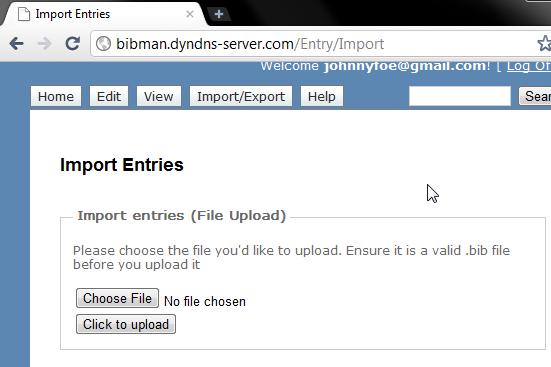
\includegraphics
			[scale=0.6]
			{images/ImportEntriesURL.png}
		\caption{Sample of a URL in used in the system}
		\label{fig:ImportEntriesURL}
	\end{center}
\end{figure}

\begin{figure}
	\begin{center}
			\lstset{language=CSharp} 
			\begin{lstlisting}
	Entry.Article, new Dictionary<Field, bool>
	 {	//Field name		Is it required?
	     {Field.Author, true}, 	// The author is required
	     {Field.Title, 	true},	// The Title is required
	     {Field.Journal,true},	// The Journal is required
	     {Field.Year, 	true},	// The Year is required

	     {Field.TheKey, false},	// The Key is optional
	     {Field.Volume, false},	// The Volume is optional
	     {Field.Number, false},	// The Number is optional
	     {Field.Pages, 	false},	// The Pages field is optional
	     {Field.Month, 	false},	// The Month is optional
	     {Field.Note, 	false},	// The Note is optional
	     {Field.Annote, false}	// The Annote field is optional
	 }
  		\end{lstlisting}
		\caption{An example dictionary entry from the \texttt{EntryFieldUsage} dictionary from \texttt{PublicationFactory}.}
		\label{fig:EntryFieldUsage}
	\end{center}
\end{figure}
\begin{figure}
	\begin{center}
			\lstset{language=CSharp} 
			\begin{lstlisting}
	...
	// get the information on which to base decisions
	Dictionary<Field, bool> dict = PublicationFactory.EntryFieldUsage[EntryType];
	const string commaNewlineIndent = ",\r\n  ";
	// construct the start of the BibTeX-formatted entry
	string retVal = "@" + EntryType + "{" + CiteKey;
	bool discardedBoolean;
	// if the author field is in the dictionary, 
	// then it is a field associated with the entry type.  
	
	// if it is null/empty, it is not required and can be omitted
	if (dict.TryGetValue(Field.Author, out discardedBoolean) && !String.IsNullOrEmpty(Authors))
	{
	    retVal += commaNewlineIndent + "Author = {" + Authors + "}";
	}
	// and so on for all possible fields
	... 
	return retVal
  		\end{lstlisting}
		\caption{A sample of conversion to the BibTeX format for the `Author' field}
		\label{fig:BibFileConversion}
	\end{center}
\end{figure}



\subsection{Search}
\label{searchCore}
The search is facilitated by the \texttt{DataPersistence} class, by way of the\\ \texttt{GetActivePublicationsMatching(searchString)} method.  

\begin{enumerate}
	\item Firstly, the \texttt{string} is prepared for the database, to allow for wildcards;
	\item Secondly, the search is carried out across the database;
	\item Thirdly, results are collated to \cs's List type and returned for use by the calling method.
\end{enumerate}

Users search by strings, which can include the wildcards '*' for any sequence of characters and '?' for any single character.
This is facilitated by the method entitled \texttt{PrepareSqlString} in the \texttt{DataPersistence} class as shown in Figure \ref{fig:SQLsearchEscape}.

\begin{figure}
	\begin{center}
			\lstset{language=CSharp} 
			\begin{lstlisting}
  private static string PrepareSqlString(string s)
  {
      // escapes SQL wildcards and inserts SQL wildcards in
      // place of characters * and ?
      
      // check for % signs and replace with \%
      s = Regex.Replace(s, "%", "\\%");
      // Check for * signs and replace with %
      s = Regex.Replace(s, "\\*", "%");
      // Check for _ signs and replace with \_
      s = Regex.Replace(s, "_", "\\_");
      // check for ? signs and replace with _
      s = Regex.Replace(s, "\\?", "_");
      return s;
  }
  		\end{lstlisting}
		\caption{Code to escape SQL wildcards and convert asterisks and question marks into SQL-query friendly strings}
		\label{fig:SQLsearchEscape}
	\end{center}
\end{figure}

The search is performed by the method in the \texttt{DataPersistence} class entitled \texttt{GetActivePublicationsMatching(string s)}, which can be seen in Figure \ref{fig:PerformSearch}.  This code snippet is a good example of how the strongly-typed, \gls{oo} queries (benefits of NHibernate mentioned in \ref{nhibernate}) are used effectively and efficiently.  They are written in \gls{linq}, a language which addresses the needs of developers by enabling support directly in the programming language \cite{csUnleashed}.

\begin{figure}
	\begin{center}
			\lstset{language=CSharp} 
			\begin{lstlisting}
	public static IList<Publication> GetActivePublicationsMatching(string s)
	{
	    // prepare the SQL string - escape SQL wildcards 
	    //         and replace * and ? characters
	    s = PrepareSqlString(s);
	    
	    // Get a session with the database
	    var currentSession = GetSession();
	
	    // Put together the search query in LINQ and execute it
	    var a = from pub in currentSession.Linq<Publication>()
	            where pub.DeletionTime == null &&
	                  (pub.CiteKey.Contains(s) ||
	                  pub.Address.Contains(s) ||
	                  pub.Annote.Contains(s) ||
	                  pub.Authors.Contains(s) ||
	                  pub.Booktitle.Contains(s) ||
	                  pub.Chapter.Contains(s) ||
	                  pub.Crossref.Contains(s) ||
	                  pub.Edition.Contains(s) ||
	                  pub.Editors.Contains(s) ||
	                  pub.Howpublished.Contains(s) ||
	                  pub.Institution.Contains(s) ||
	                  pub.Journal.Contains(s) ||
	                  pub.TheKey.Contains(s) ||
	                  pub.Month.Contains(s) ||
	                  pub.Note.Contains(s) ||
	                  pub.Number.Contains(s) ||
	                  pub.Organization.Contains(s) ||
	                  pub.Pages.Contains(s) ||
	                  pub.Publisher.Contains(s) ||
	                  pub.School.Contains(s) ||
	                  pub.Series.Contains(s) ||
	                  pub.Title.Contains(s) ||
	                  pub.Type.Contains(s) ||
	                  pub.Volume.Contains(s) ||
	                  pub.Year.Contains(s))
	            select pub;
	
	    // convert the results to a list and return them
	    return a.ToList();
	}  		
			\end{lstlisting}
		\caption{Code to perform a search}
		\label{fig:PerformSearch}
	\end{center}
\end{figure}


\section{Web Service}
\label{webService}
The project has several areas which are performed by \gls{ajax} interactions with the system.  These interactions are handled by a web service entitled \texttt{SearchResults}. It was initially intended to handle only the instant search result collation; refactoring was attempted to rename the service to a more representative name, but there were too many issues with the name change, hence the slightly misleading name.

The instant search function is supported by a web service which accepts a search \texttt{string}, performs a search on the database by reusing the search method discussed in Section~\ref{searchCore}, and returns the results in a \gls{json} array, for the client-side code (\gls{js}) to deal with.  

Delete functionality and duplicate reduction functionality are both provided by \gls{ajax} requests by calls to the \texttt{DeletePublication(int id)} method of the web service.  It again reuses the \texttt{DataPersistence} class's method of the same name to mark an entry in the system as deleted, before returning the result to the client.

A deleted entry (see Section~\ref{dataModel} for the model's definition of `deleted') is timestamped with the time of its deletion, which can be used to determine entries which have been deleted since a given time by comparing the given time with the deletion time. 

The web services provides a behind-the-scenes ability to find out what entries have been deleted since a given time.  This core code which performs the result accumulation is shown in Figure \ref{fig:getDeletedPublicationsWS}; some of the code, particularly exception-handling clauses, is excluded here for brevity.

\begin{figure}
	\begin{center}
			\lstset{language=CSharp} 
			\begin{lstlisting}
  // Parse the given creation time into a DateTime object
  DateTime d = DateTime.Parse(pageCreationTime);

  // Get deleted entries into a list
  var pubs = (from publications in DataPersistence.GetSession().Linq<Publication>()
              select publications).ToList();
  pubs = pubs.Where(p => (p.DeletionTime.HasValue)).ToList();

  // create the list of results
  IList<int> result = new List<int>();
  foreach (Publication publication in pubs)
  {
      if (publication.DeletionTime != null)
          // if the deletion time is newer than DateTime d, add it to the return list.
          if (publication.DeletionTime.Value.CompareTo(d) > 0)
              result.Add(publication.Id);
  }

  return result;
			\end{lstlisting}
		\caption{Code to retrieve deleted entries since a given time}
		\label{fig:getDeletedPublicationsWS}
	\end{center}
\end{figure}

This approach is used to facilitate concurrent access by notification that items have been changed in the system.  

Similarly to the way deleted entries' times are tracked, the amendment and creation times of an entry is tracked by a field entitled `AmendmentTime' and `CreationTime' respectively.  A list of recently-amended or created entries can be accumulated by the same algorithm as for deleted entries.

The use of these web services in the concurrent access aspect of the system is discussed fully in Section~\ref{concurrency}.

\section{View}
The views of the project were implemented in \gls{asp}\gls{net}, which is effectively a mixture of \gls{html} and \cs{} server-side code.  Each view is strongly-typed to a particular class, which results in swift development that is checked at compile-time, resulting in type-safe code.

Discussing each view in its entirety would not be conducive to a reader's understanding.  Instead, several key pages are discussed, in particular:
\begin{enumerate}
	\item The \texttt{Publication} creation and modification page;
	\item The `View all entries' page;
	\item The `Search' page, in particular the instant search functionality;
\end{enumerate}

Each of these pages' descriptions will give a vision of what the result is, followed by the code used 

\subsection{Publication}
\label{pubPage}
To ensure a consistent experience for the user, one page serves two data-input functions: firstly to create a new valid entry and secondly to amend an existing entry.

When a user wants to create an entry, they will have navigated to the \texttt{Publication} \gls{url}.  This \gls{url} will be \url{http://bibman.dyndns-server.com/Entry/Publication}, as an example.  The controller handles checking of the \gls{url} for an Id, which would suggest that the entry already exists.  The controller then returns an empty version of the page to the client, which appears as shown in Figure~\ref{fig:PublicationLandingPage}.

\begin{figure}
	\begin{center}
		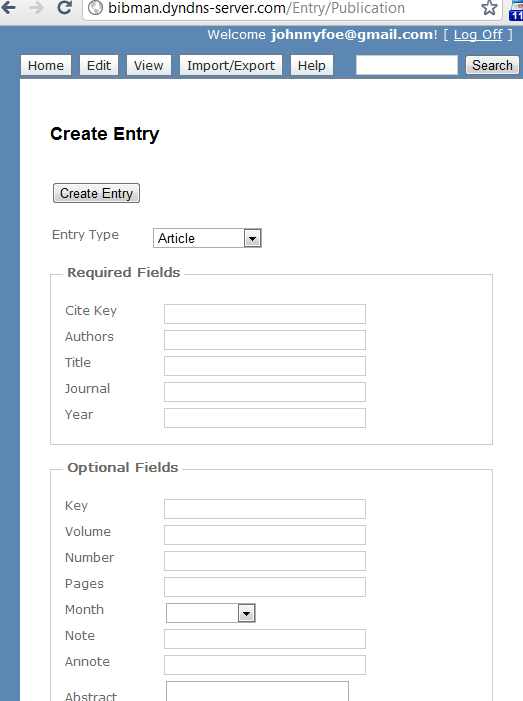
\includegraphics
			[scale=0.45]
			{images/PublicationLandingPage.png}
		\caption{Publication page -- initial view}
		\label{fig:PublicationLandingPage}
	\end{center}
\end{figure}

When the user selects the drop down box as shown in Figure~\ref{fig:DropDownInBook} and subsequently chooses a value, the result is that the fields which are required and optional are moved to suit the entry type as shown in Figure~\ref{fig:InbookChanged}

\begin{figure}
	\begin{center}
		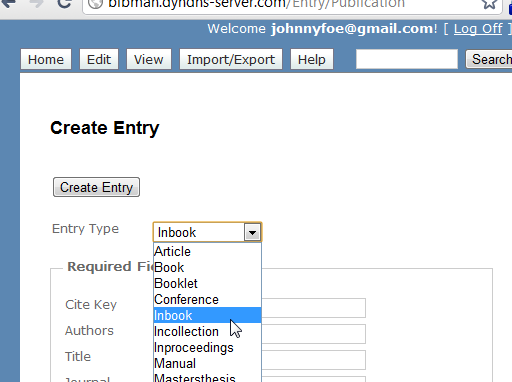
\includegraphics
			[scale=0.45]
			{images/DropDownInBook.png}
		\caption{Drop Down box with InBook as target}
		\label{fig:DropDownInBook}
	\end{center}
\end{figure}

\begin{figure}
	\begin{center}
		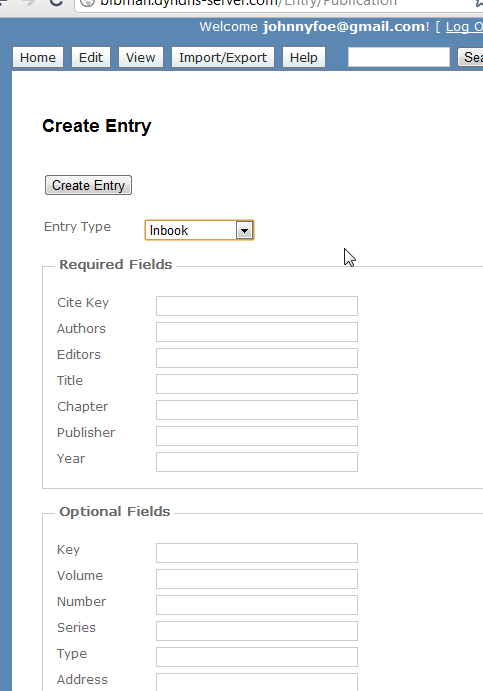
\includegraphics
			[scale=0.45]
			{images/InbookChanged.png}
		\caption{Drop Down box changed to InBook}
		\label{fig:InbookChanged}
	\end{center}
\end{figure}

This change is achieved by use of \gls{js}, which is fired on every change made to the entry type drop down box.  In effect, the \gls{js} moves all required, optional and unused fields to a ``required'' fieldset, an ``optional'' fieldset and a ``hidden'' div.  A benefit of this approach is that if a user mis-clicks the drop down entry, any information that they have entered will not be lost, as it will still exist in the hidden div.  The structure of the code is outlined in the source code shown in Figure~\ref{fig:PublicationSourceCode} and shows the two displayed fieldsets and the ``hidingPlace'' div.  A sample of the \gls{js} used to achieve this is given in Figure~\ref{fig:SwitchOutFields}.  

\begin{figure}
	\begin{center}
		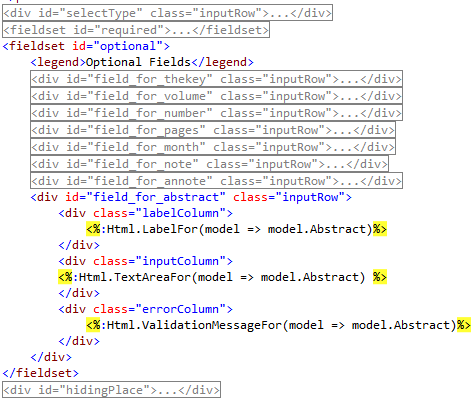
\includegraphics
			[scale=0.7]
			{images/PublicationSourceCode.png}
		\caption{Source code of the Publication View}
		\label{fig:PublicationSourceCode}
	\end{center}
\end{figure}

\begin{figure}
	\begin{center}
			\lstset{language=JavaScript} 
			\begin{lstlisting}
function ChangeEntryType() {

  ...

  var required = document.getElementById('required'); /* required Fieldset */
  var optional = document.getElementById('optional'); /* optional Fieldset */
  var hidden = document.getElementById('hidingPlace'); /* hiding place for unused fields*/

  var abstract = document.getElementById('field_for_abstract');
  var citekey = document.getElementById('field_for_citekey');

  var address = document.getElementById('field_for_address');
  
  /* ... and so on for all fields */
  
  var year = document.getElementById('field_for_year');

  required.appendChild(citekey);
		
		...
		
  else if (entryType == "Inbook") {
    required.appendChild(author);
    required.appendChild(editor);
    required.appendChild(title);
    required.appendChild(chapter);
    required.appendChild(publisher);
    required.appendChild(year);

    optional.appendChild(key);
    optional.appendChild(volume);
    optional.appendChild(number);
    optional.appendChild(series);
    optional.appendChild(type);
    optional.appendChild(address);
    optional.appendChild(edition);
    optional.appendChild(month);
    optional.appendChild(pages);
    optional.appendChild(note);
    optional.appendChild(annote);

    hidden.appendChild(booktitle);
    hidden.appendChild(crossref);
    hidden.appendChild(howpublished);
    hidden.appendChild(institution);
    hidden.appendChild(journal);
    hidden.appendChild(organization);
    hidden.appendChild(school);
  }
}
			\end{lstlisting}
		\caption{Code to retrieve move fields between Required, Optional and Hidden field sets}
		\label{fig:SwitchOutFields}
	\end{center}
\end{figure}

As was mentioned at the beginning of this section, this approach is used for both the amendment and creation phases of entries.  When the controller is supplied with an Id, it tries to fetch the entry associated with it from the database.  If an entry is found, it must be displayed in a consistent manner with the way entries are displayed in the creation stage.

There are some differences between the creation page and the amendment page, which are highlighted in Figure~\ref{fig:amendAndCreate}.  Firstly, the pages are clearly marked with different titles and names on the submission buttons.  Secondly, the amendment page has pre-selected the entry type and displayed the fields for it.  Thirdly, an option to delete the entry that exists has appeared.  Each of these changes makes it clear to a user what the options available to them are at all times, while maintaining excellent consistency of both behaviour and display across the two pieces of functionality.

\begin{figure}
	\begin{center}
		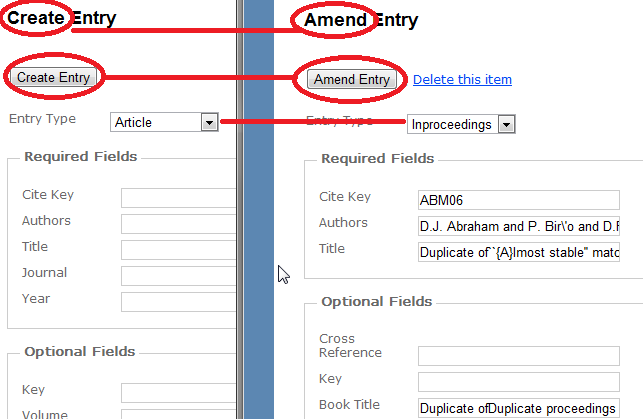
\includegraphics
			[scale=0.7]
			{images/amendAndCreate.png}
		\caption{Amendment and Creation pages side-by-side}
		\label{fig:amendAndCreate}
	\end{center}
\end{figure}

Users are given clear feedback in the view section which ensures that any entry stored adheres to non-functional requirement 9 (only valid entries can be stored).  This is seen in Figure~\ref{fig:Validation}.

\begin{figure}
	\begin{center}
		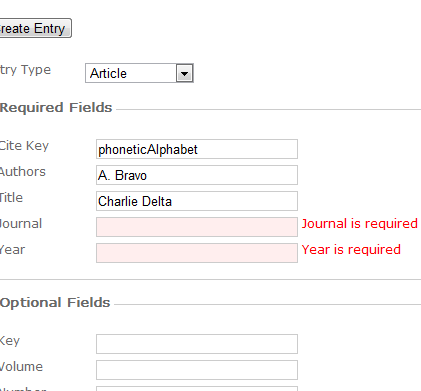
\includegraphics
			[scale=0.7]
			{images/Validation.png}
		\caption{Validation messages when an erroneous entry is submitted}
		\label{fig:Validation}
	\end{center}
\end{figure}

As discussed in Section~\ref{concurrency}, concurrent access is an issue which must be taken care of.  Recall that it is important to keep a user informed about changes to an entry when it is of interest to the user.  An example of this is when a user is viewing an entry on the amendment page.

The system deals with this by providing messages similar to those that appear in Figures~\ref{fig:ChangedPub} and \ref{fig:amendedPub}.  The implementation of these messages' delivery is discussed presently.  \gls{ajax} requests are sent periodically to the server's web service to find out if there has been a change to the entry of interest.  If there has been a change, the server responds with an appropriately coded message, which is dealt with by the \gls{js} in Figure~\ref{fig:PublicationAjaxUpdate}, resulting in the message seen in either Figure~\ref{fig:ChangedPub} or Figure~\ref{fig:amendedPub}

\begin{figure}
	\begin{center}
		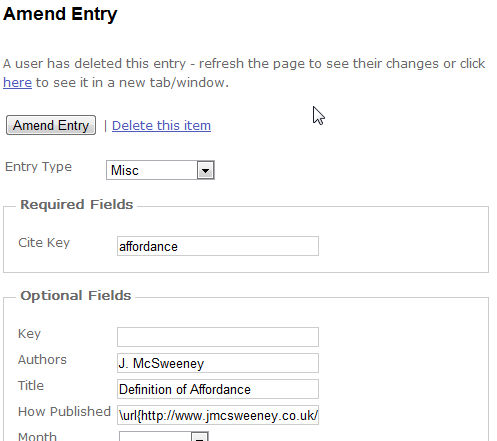
\includegraphics
			[scale=0.7]
			{images/ChangedPub.png}
		\caption{The message displayed when a publication is deleted and it is of interest to a user}
		\label{fig:ChangedPub}
	\end{center}
\end{figure}

\begin{figure}
	\begin{center}
		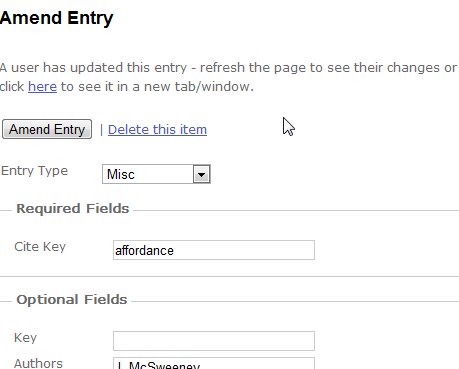
\includegraphics
			[scale=0.7]
			{images/amendedPub.png}
		\caption{The message displayed when a publication is amended and it is of interest to a user}
		\label{fig:amendedPub}
	\end{center}
\end{figure}

\begin{figure}
	\begin{center}
			\lstset{language=JavaScript} 
			\begin{lstlisting}
function CheckForModifications() {
  var createdAt = document.getElementById("PageCreationTime").value;
  var service = new BibtexEntryManager.SearchResults();
  var queryString = createdAt + " " + ItemId();
  service.HasPublicationChanged(queryString, onModificationCheckSuccess, null, null);
}

function onModificationCheckSuccess(result) {
	// entry does not exist in the db and cannot have changed.
  if (result == -1) {
    return;
  }
  // 0 signifies no change since page load
  if (result == 0) {
    // continue checking for modifications if there was 
    // no change (set the timer for another 3 seconds)
    var t = setTimeout("CheckForModifications()", 3000);
    return;
  }
  // 1 signifies deletion since page load - set the message to inform the user
  if (result == 1) {
    document.getElementById("notificationOfUpdate").innerHTML =
      "A user has deleted this entry - refresh the page to " +
      "see their changes or click <a href=\"/Entry/Publication/" +
      ItemId() + "\" target=\"_blank\">here</a> to see it in a new tab/window.";
    return;
  }
  // 2 signifies amendment since page load - set the message to inform the user
  if (result == 2) {
    document.getElementById("notificationOfUpdate").innerHTML =
      "A user has updated this entry - refresh the page to " +
      "see their changes or click <a href=\"/Entry/Publication/" +
      ItemId() + "\" target=\"_blank\">here</a> to see it in a new tab/window.";
    return;
  }
}
			\end{lstlisting}
		\caption{JavaScript used to check and manage concurrent access while on this page}
		\label{fig:PublicationAjaxUpdate}
	\end{center}
\end{figure}

% =============================================================================================
% =============================================================================================
% =============================================================================================
% =============================================================================================
% =============================================================================================
% =============================================================================================

\subsection{The `View all entries' page}
The \texttt{EntryController} index page allows the user to view all of the entries in the system.  It uses a method from the \texttt{DataPersistence} class called \texttt{GetActivePublications()}, which returns all entries in the system which have a null value for their \texttt{DeletionTime}.  Recall that if an entry has a non-null deletion time, then it is said to be deleted and inactive in the system.  Each of these entries is in turn converted using the \texttt{ToHtmlRowWithLinks()} method of the \texttt{Publication} class.  A screenshot of the list of all active entries page can be seen in Figure~\ref{fig:listallentries}.  As can be seen from the screenshot, there are clear instructions to the user on what can be performed next and what action they need to take next to perform it.

\begin{figure}
	\begin{center}
		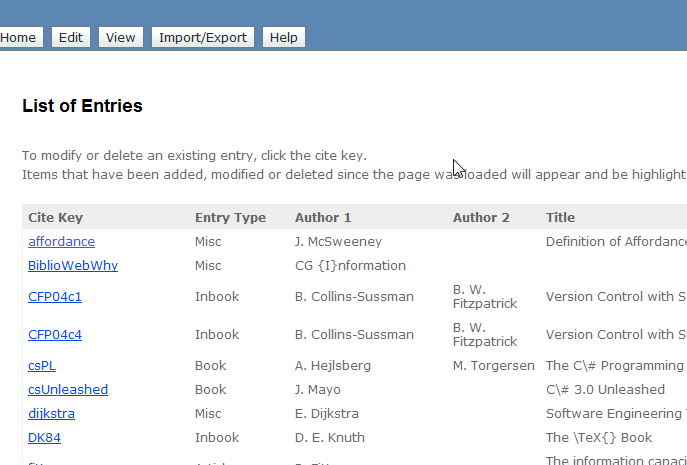
\includegraphics
			[scale=0.7]
			{images/listallentries.png}
		\caption{The list of all entries in its initial state}
		\label{fig:listallentries}
	\end{center}
\end{figure}

Columns can be sorted by clicking on any of the field name headers, as shown in Figure~\ref{fig:sorted}.  This is accomplished by use of the sorttable \gls{js} library, which was kindly made open by Stuart Langridge\footnote{Stuart Langridge's product and more information about it can be found at  \url{http://www.kryogenix.org/code/browser/sorttable/}}.  By pushing the sorting of entries out to clients, the load on the server is reduced, because the server does not need to deal with the computational requirements of sorting the set of all entries.  There is a drawback with this system if the client machine is not very computationally powerful or the list of entries is particularly large.  In these cases, sorting takes a noticeable time.  To get around this, future versions of the program should either introduce paging or keep all sorting of entries on the server-side.

\begin{figure}
	\begin{center}
		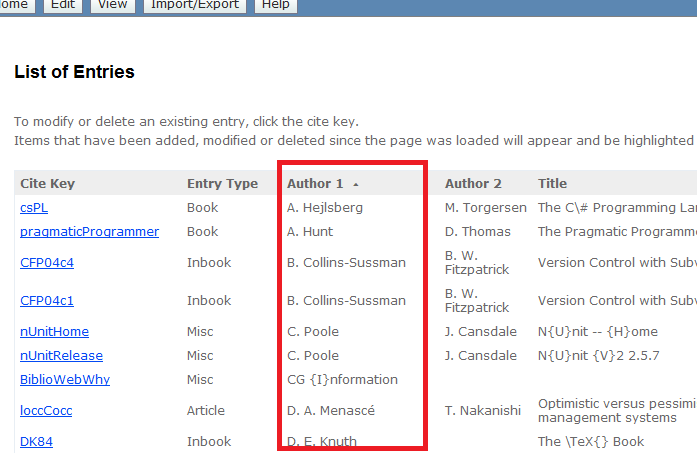
\includegraphics
			[scale=0.7]
			{images/sorted.png}
		\caption{The list of all entries sorted by a different column (highlighted)}
		\label{fig:sorted}
	\end{center}
\end{figure}

Concurrent access issues are dealt with in a similar way to the way that they were dealt with in Section~\ref{pubPage}.  The page periodically polls the server to find out if there have been changes to the entries of interest since the page was loaded. It then makes updates to the display when changes have been made.  Red is used to symbolise the deletion of an entry; yellow is used to symbolise the modification of an entry, and green is used when a new entry is added.  These colours can be seen in Figure~\ref{fig:ConcurrencyColours}.  
\begin{figure}
	\begin{center}
		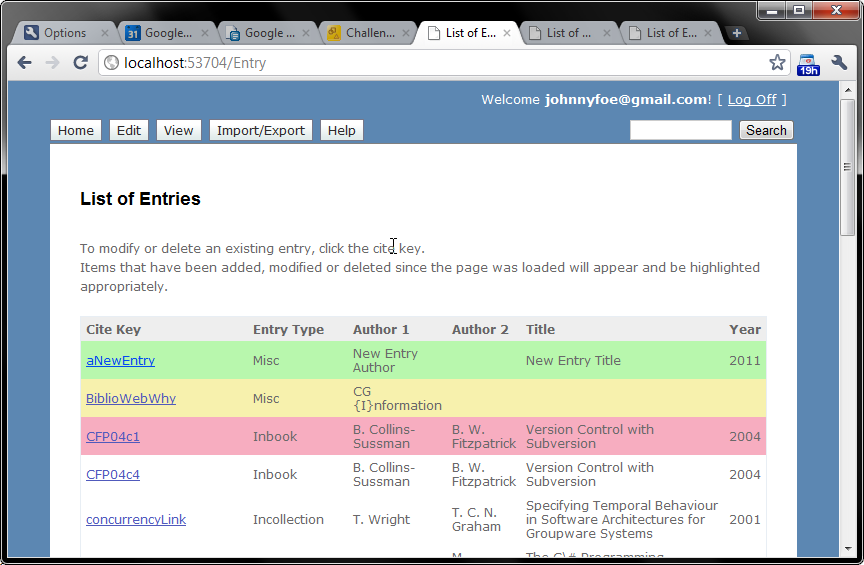
\includegraphics
			[scale=0.7]
			{images/ConcurrencyColours.png}
		\caption{The list of all entries with concurrent access facilitation features shown}
		\label{fig:ConcurrencyColours}
	\end{center}
\end{figure}

The \gls{js} client-side code to send \gls{ajax} requests and handle \gls{json} responses is shown in Figure~\ref{fig:listAjaxUpdate}.  This code is assisted by Microsoft's \gls{net} framework which abstracts the representation of the web service to a name, as can be seen in the third line of the code in Figure~\ref{fig:listAjaxUpdate}.

\begin{figure}
	\begin{center}
			\lstset{language=JavaScript} 
			\begin{lstlisting}
function UpdateContent() {
  var createdAt = document.getElementById("PageCreationTime").value;
  var service = new BibtexEntryManager.SearchResults();
  // send requests to the server.  
  service.GetAmendedPublications(createdAt, onAmendmentCheckSuccess, null, null);
  service.GetDeletedPublications(createdAt, onDeletedItemsCheckSuccess, null, null);
  service.GetNewPublications(createdAt, onNewPublicationsCheckSuccess, null, null);

  var currentDate = new Date();

  document.getElementById('PageCreationTime').value = currentDate.toGMTString();
  timeUpdateContent(); // poll server every 3 seconds
}
// Executed when amended publications' ids are returned successfully
function onAmendmentCheckSuccess(result) {
  if (result != null) {
    for (var i = 0; i < result.length; i++) {
      document.getElementById("tr_" + result[i]).setAttribute("class", "AmendedPublication");
    }
  }
}
// Executed when deleted publications' ids are returned successfully
function onDeletedItemsCheckSuccess(result) {
  if (result != null) {
    for (var i = 0; i < result.length; i++) {
      document.getElementById("tr_" + result[i]).setAttribute("class", "DeletedPublication");
    }
  }
}
// Executed when new publications are returned successfully
function onNewPublicationsCheckSuccess(result) {
  if (result != null) {
    var tbodies = document.getElementsByTagName("tbody");
    var originalHTML = tbodies[0].innerHTML;
    var finalString = "";
    for (var k = 0; k < result.length; k++) {
      finalString += result[k];
    }
    tbodies[0].innerHTML = finalString + originalHTML;
  }
}
			\end{lstlisting}
		\caption{JavaScript code used to update the list of all entries by AJAX requests}
		\label{fig:listAjaxUpdate}
	\end{center}
\end{figure}

\subsection{Instant Search}
There is a consistent `Search' feature in the top-right hand corner of every page below the log in area.  Submission of a search value into this box will return the list of entries that matches the search term provided.  This search functionality, along with the function described next, uses the same core search method set discussed in Section~\ref{searchCore}.

Searching with the search box returns a set of results displayed thus:
\begin{figure}
	\begin{center}
		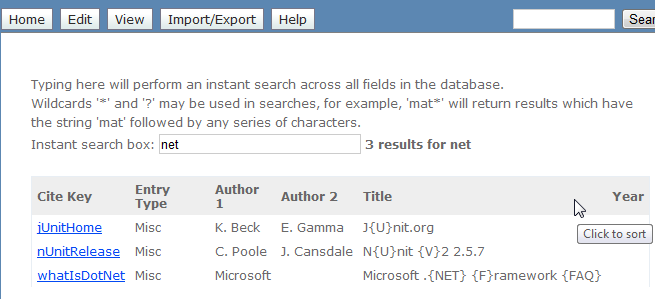
\includegraphics
			[scale=0.7]
			{images/searchNormal.png}
		\caption{Initial search results for a query}
		\label{fig:searchNormal}
	\end{center}
\end{figure}
Notice that there is clear feedback on the size of the result set returned, along with clear instruction on what functionality is provided by this page.

The instant search box updates on every key press.  The progress of a simple query is outlined by Figures~\ref{fig:instant1} and \ref{fig:instant2}.
\begin{figure}
	\begin{center}
		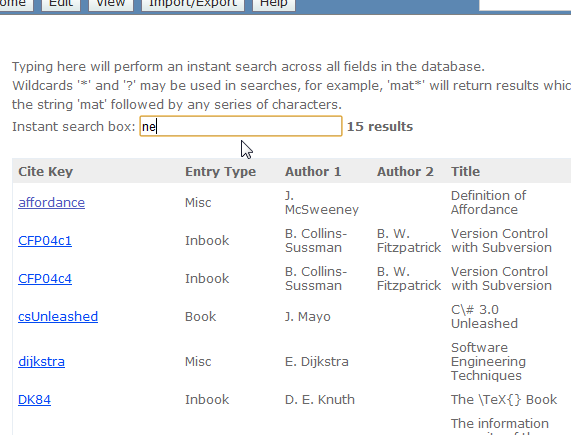
\includegraphics
			[scale=0.7]
			{images/instant1.png}
		\caption{Search results after the backspace key was pressed once}
		\label{fig:instant1}
	\end{center}
\end{figure}

\begin{figure}
	\begin{center}
		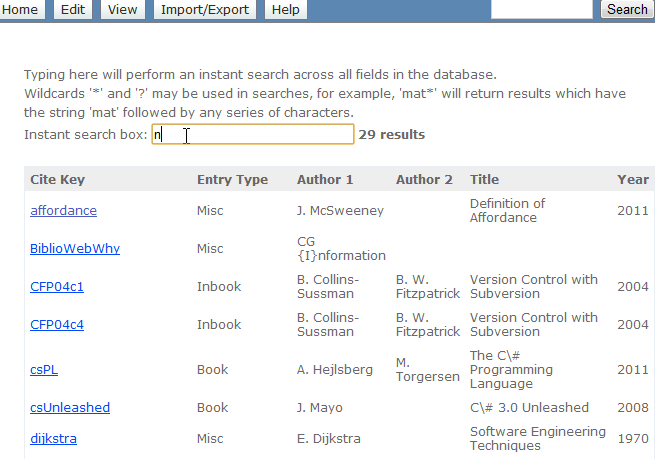
\includegraphics
			[scale=0.7]
			{images/instant2.png}
		\caption{Search results after the backspace key was pressed a further time}
		\label{fig:instant2}
	\end{center}
\end{figure}

The instant search is facilitated again by \gls{ajax} requests and the web service discussed in Section~\ref{webService}.  Each time a key is pressed, a request is sent to the server for search results.  When the request is received, the \texttt{DataPersistence} class is queried as laid out at the beginning of this section.  The result is passed back to the client as an array in \gls{json}.  

This result is then inserted into the search results table if there are results to be shown, or a message is inserted to alert users to the lack of results.  The message to the right of the instant search box is also updated on receipt of the response to alert users to the number of results for the query they have typed.

A snapshot of the code used by this approach is shown in Figure~\ref{fig:instaSearch}.

\begin{figure}
	\begin{center}
			\lstset{language=html} 
			\begin{lstlisting}
<input id="searchString" type="text" onkeyup="return keysearch()" /> 
			\end{lstlisting}
		\caption{HTML which is used to fire the AJAX request after each key-up event}
		\label{fig:html}
	\end{center}
\end{figure}

\begin{figure}
	\begin{center}
			\lstset{language=JavaScript} 
			\begin{lstlisting}
function keysearch() {
  var service = new BibtexEntryManager.SearchResults();
  service.DoSearchRaw(document.getElementById("searchString").value, onSuccess, null, null);
}

function onSuccess(result) {
  document.getElementById("searchCount").innerHTML = (result != null) ? result.length + " result" + ((result.length != 1) ? "s" : "") : "";
  if (result.length > 0) {
    var s = "";
    for (var i = 0; i < result.length; i++) {
      s += result[i];
    }
    document.getElementById("results").innerHTML = s;
    sorttable.makeSortable(document.getElementsByTagName("table")[0]);
  }
  else {
    document.getElementById("results").innerHTML = "<tr><td>There are no results.</td></tr>";
  }
}
			\end{lstlisting}
		\caption{JavaScript code used to update the list of all entries by AJAX requests}
		\label{fig:instaSearch}
	\end{center}
\end{figure}
 
\glsreset{ui}
\subsection{Consistency}
The consistency sought in the design of the product (see Section \ref{uiDesign}) of the site is a result of careful consideration of what should be consistent across all pages, as highlighted in Figure \ref{fig:pageLayout}, which has certain features annotated numerically as follows:

\begin{figure}
	\begin{center}
		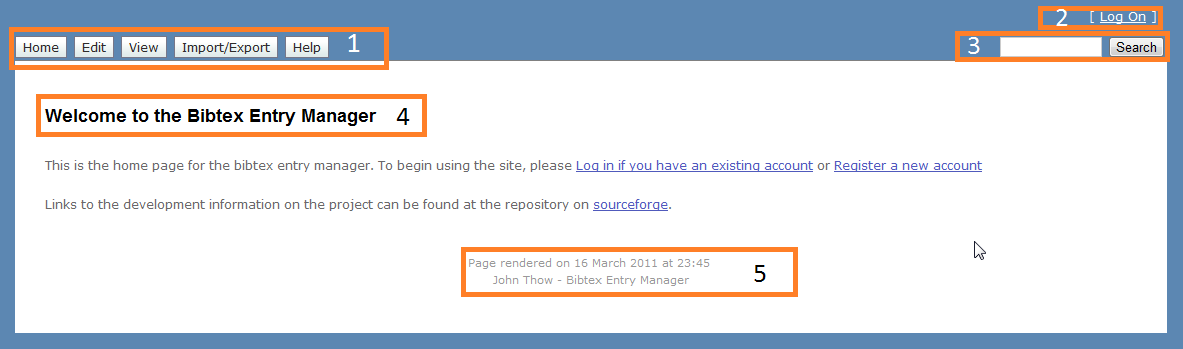
\includegraphics
			[scale=0.5]
			{images/PageLayout.png}
		\caption{Annotation of a page}
		\label{fig:pageLayout}
	\end{center}
\end{figure}

\begin{figure}
	\begin{center}
		
\includegraphics
			{images/LogOff.png}
		\caption{The log on area when a user is logged in (swapped out for area 2 in Figure \ref{fig:pageLayout})}
		\label{fig:logOff}
	\end{center}
\end{figure}

\begin{enumerate}
	\item Firstly, there is a menu area which appears on every page within the site, with the same options at each appearance.  This gives the user a single point of reference to aid while navigating the website;
	\item The log on area appears in one of two forms across all pages of the application: a user is either browsing anonymously, or is logged in.  It is clear which of these two states the user's session is in thanks to the clear representation of the words `Log On' (depicted in Figure \ref{fig:pageLayout}) and a welcome message with the current user's email address (as depicted in Figure \ref{fig:logOff})
	\item After feedback from a user during the basic evaluation (see Chapter \ref{eval}) the interface was updated to include a search area on all pages.  The provision of this area allows a user to efficiently search the system's database for a string with no further navigation.  It also provides users with a further concrete point of reference, which adds to the consistency of the interface.
	\item Each and every page contains a bold header indicating the title of the page.  The presence of a title on each page gives a user another concrete and consistent place to glance in order to gain an insight into what they previously clicked on, as well as giving confirmation that their previous action was successful.
	\item The fifth item highlighted in this image provides some extra, arguably unnecessary information.  The main idea behind including this page render time area is to provide extra feedback: it lets a user know that page has finished loading, that it has been completed successfully and it reassures a user that the page is up to date.
\end{enumerate}

This consistency was implemented using a feature in \gls{asp}\gls{net} called ``Master Pages''.  As the name suggests, the developer creates a master page with the main layout of the website, within which sit containers which are filled by individual pages.  This approach centralises the code for the pages.  The advantages of centralising code are discussed in Section \ref{codeReuse}.

The colour choice of the interface was a decision which was postponed until later in the project, so that the bulk of the development work could be carried out before aesthetics were considered.  The colour scheme seen in the project is based on the default style for projects created in \gls{msvs} 2010; it soon became apparent that the default style had many strong qualities that could be used as the main theme for the web site.  Consequently, the colour scheme was retained and extra features were built around it.



\section{Development Environment}
\label{devEnv}
Most of the development took place on the developer's laptop, a MacBook Pro dual-booted with Windows 7 Professional.  Some development took place on a second developer machine when the laptop was unavailable.

The main development environment was Microsoft's Visual Studio Professional 2010 (\gls{msvs}), provided by the School's \gls{msdnaa} agreement.  This was the same environment used while on summer placement, so the developer was familiar with the tools in the \gls{ide}.

The database product used was \gls{msss} 2008 Developer Edition, again provided by the School's \gls{msdnaa} agreement. The management suite included with the product was again used while on summer placement, and the developer was familiar with the tools in the program.

ReSharper is a productivity plug-in for \gls{msvs}.  It provides code inspections, code analysis, one-click unit test runs (see Figure~\ref{fig:NUnitTestRunner}, project-level refactorings and many more assistive features.  A licence for the product was purchased during the summer placement and was used extensively throughout the development of the software article.

\begin{figure}
	\begin{center}
		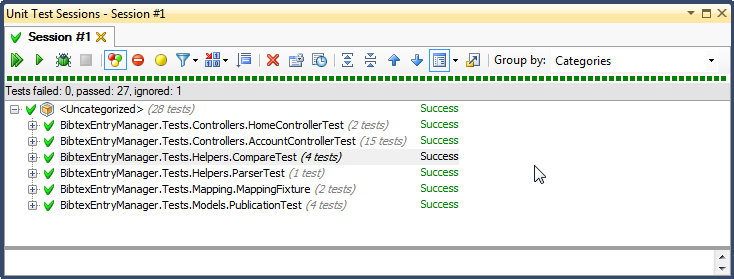
\includegraphics
			[scale=0.45]
			{images/NUnitTestRunner.png}
		\caption{NUnit One-Click Test Runner, part of the ReSharper plug-in}
		\label{fig:NUnitTestRunner}
	\end{center}
\end{figure}

Python IDLE and Notepad++ were used to manipulate code quickly and effectively: Python IDLE for its scripting functionality and Notepad++ for its macro capabilities and excellent search and replace by regular expression function.

TortoiseSVN and AnkhSVN were both used as discussed in Section \ref{svn}.

\section{Subversion}
\glsreset{svn}
\label{svn}
\gls{svn} is a centrally-stored version control system which records every change ever made to the files and directories in the file repository \cite{CFP04c1}.  It is useful to be able to centralise the code repository and to be able to synchronise different workstations with the most up to date version of code and documents, as well as allowing the logging and comparison of different versions of the code.  

Each time information is updated in the repository, it is said to have a new revision -- a process also known as `committing' changes.  It was decided early in the project that a repository would be used to mitigate the risk of fire, flood, theft, and hard drive corruption by hosting the repository in a different physical location to the main work environment, the developer's laptop.  

\gls{svn} was used to control different versions of the code and to take snapshots of the project in the form of \gls{svntag}s \cite{CFP04c4}, as well as normal revisions.  It was originally hosted on the School of Computing Science network because it was accessible from outside the School's network of computers\footnote{access was facilitated by the School's \gls{ssh} gateway, \texttt{sibu.dcs.gla.ac.uk}}, because there was sufficient storage space provided by the School and it had no financial cost.  

As part of the effort to ensure good software engineering practice, \gls{ci}\footnote{See Section \ref{continuousIntegration} for an explanation of what it is and why it was used} was to be used with the project.  It was another technology encountered on summer placement.  Unfortunately, there were problems in configuring the \gls{ci}  software to access the \gls{svn} repository through the gateway; as a result of this, on the 16\^{th} of November 2010, the repository was moved to another free host, SourceForge, an open-source software project hosting provider.  

Along with \gls{svn} repository hosting, SourceForge provides tools for management of software projects, including a bug tracking tool (see Section \ref{bugTracking}).  Crucially, the SourceForge repository was accessible by the \gls{ci} software, allowing the \gls{ci} process to take place.  The \gls{ci} process is discussed in detail in Section \ref{continuousIntegration}.

The \gls{svn} client in most cases was TortoiseSVN, as development was to take place on a windows environment.  AnkhSVN, a secondary client, was also used as it integrated with the \gls{msvs} \gls{ide}. 

The repository can be browsed on the SourceForge website at \url{http://bibman.svn.sourceforge.net/}

\section{Summary of Implementation}
Many techniques and technologies have been employed, encountered and learned about during the implementation of the software solution.  It is hoped that the information within this chapter gave a good insight into some of the activity during the implementation of the system.

The next chapter discusses the approach that was taken to testing the solution. It focusses on the technologies used and the discipline applied during testing of the software.